\documentclass[tikz,border=10pt]{standalone}
\usepackage{tikz}
\usetikzlibrary{arrows.meta,calc}

\definecolor{figazul}{RGB}{2,132,199}
\definecolor{figrojo}{RGB}{220,38,38}
\definecolor{figverde}{RGB}{22,163,74}

\begin{document}
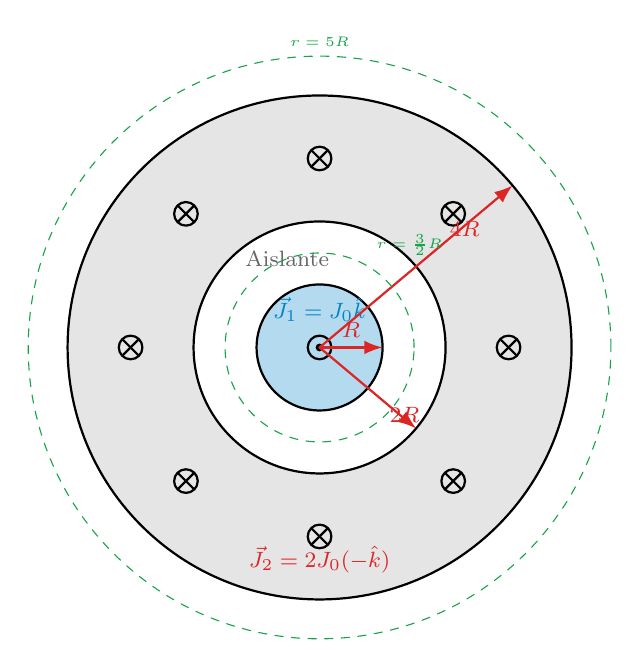
\begin{tikzpicture}[>=Latex, line cap=round, line join=round]
  % Cascarón exterior: 2R = 1.6, 4R = 3.2
  \draw[thick, fill=gray!20] (0,0) circle (3.2);
  \draw[thick, fill=white] (0,0) circle (1.6);

  % Conductor central macizo: radio R = 0.8
  \draw[thick, fill=figazul!30] (0,0) circle (0.8);

  % Zona intermedia aislante: 0.8 < r < 1.6 (blanca)
  \node[font=\footnotesize, color=gray!80!black] at (110:1.2) {Aislante};

  % Símbolos de corriente
  % Conductor central: J1 = J0 (+z, sale)
  \draw[thick] (0,0) circle (0.15);
  \fill (0,0) circle (0.05);
  \node[above, font=\footnotesize, color=figazul] at (0, 0.2) {$\vec{J}_1 = J_0\hat{k}$};

  % Cascarón exterior: J2 = 2J0 (-z, entra: otimes)
  \foreach \ang in {0, 45, 90, 135, 180, 225, 270, 315} {
    \draw[thick] (\ang:2.4) circle (0.15);
    \draw[thick] (\ang:2.4) ++(-0.1,-0.1) -- ++(0.2,0.2);
    \draw[thick] (\ang:2.4) ++(-0.1,0.1) -- ++(0.2,-0.2);
  }
  \node[below, font=\footnotesize, color=figrojo] at (0, -2.4) {$\vec{J}_2 = 2J_0(-\hat{k})$};

  % Radios y cotas con flechas
  \draw[->, thick, color=figrojo] (0,0) -- (0:0.8);
  \node[above, color=figrojo, font=\footnotesize] at (0.4, 0) {$R$};

  \draw[->, thick, color=figrojo] (0,0) -- (-40:1.6);
  \node[below right, color=figrojo, font=\footnotesize] at (-40:1.0) {$2R$};

  \draw[->, thick, color=figrojo] (0,0) -- (40:3.2);
  \node[above right, color=figrojo, font=\footnotesize] at (40:2.0) {$4R$};

  % Lazos amperianos en r = 3R/2 (1.2) y r = 5R (4.0)
  \draw[dashed, thin, color=figverde] (0,0) circle (1.2);
  \node[above right, font=\tiny, color=figverde] at (60:1.2) {$r = \frac{3}{2}R$};

  \draw[dashed, thin, color=figverde] (0,0) circle (3.7);
  \node[above, font=\tiny, color=figverde] at (90:3.7) {$r = 5R$};
\end{tikzpicture}
\end{document}
